\documentclass[a4paper, 12pt]{article}
\usepackage[T2A]{fontenc}
\usepackage[utf8]{inputenc}
\usepackage[english,russian]{babel}
\usepackage{amsmath, amsfonts, amssymb, amsthm, mathtools, misccorr, indentfirst, multirow}
\usepackage{wrapfig}
\usepackage{graphicx}
\usepackage{subfig}
\usepackage{adjustbox}
\usepackage{pgfplots}

\usepackage{geometry}
\geometry{top=20mm}
\geometry{bottom=20mm}
\geometry{left=20mm}
\geometry{right=20mm}
\newcommand{\angstrom}{\textup{\AA}}

\title{Лабораторная работа 2.4\\Компьютерная сцинтилляционная $\gamma$-спектроскопия}
\author{Нехаев Александр, гр. 654}
\date{\today}
\begin{document}
	\maketitle
	\tableofcontents
	\section{Введение}
	\paragraph{Цель работы:}
	определить зависимость энергии и интенсивности гамма-линий от различных гамма источников и идентифицировать их.
	\paragraph{В работе используются:}
	сцинтиллятор, ФЭУ, предусилитель импульсов, высоковольтный блок питания для ФЭУ, АЦП, компьютер.
	\subsection{Теоретическое введение}
	\paragraph{Фотоэффект.}
	Это процесс взаимодействия гамма-кванта с электроном, связанным с атомом, при котором электрону передается вся энергия гамма-кванта. При этом электрону сообщается кинетическая энергия $T_e=E_\gamma-I_i$, где $E_\gamma$ -- энергия гамма-кванта, $I_i$ -- потенциал ионизации $i$-той оболочки атома. Фотоэффект особенно существенен для тяжелых веществ, где он идет с заметной вероятностью даже при высоких энергиях гамма-квантов. В легких веществах фотоэффект становится заметен лишь при относительно небольших энергиях гамма-квантов. Наряду с фотоэффектом, при котором вся энергия гамма-кванта передается атомному электрону, взаимодействие гамма-излучения со средой может приводить к его рассеянию, т.е. отклонению от первоначального направления распространения на некоторый угол.
	\paragraph{Эффект Комптона.} Это упругое рассеяние фотона на свободном электроне, сопровождающееся изменением длины волны фотона (реально этот процесс происходит на слабо связанных с атомом внешних электронах). Максимальная энергия образующихся комптоновских электронов соответствует рассеянию гамма-квантов на $180^\circ$ и равна
	\begin{equation}
		E_{\max}=\frac{\eta\omega}{1+\frac{mc^2}{2\eta\omega}}.
	\end{equation}
	\paragraph{Процесс образования электрон-позитронных пар.}
	При достаточно высокой энергии гамма-кванта наряду с фотоэффектом и эффектом Комптона может происходить третий вид взаимодействия гамма-квантов с веществом -- образование электрон-позитронных пар. Процесс образования пар не может происходить в пустоте, так как в этом случае не выполняются законы сохранения энергии и импульса. В присутствии ядра или электрона процесс образования пары гамма-квантов возможен, так как можно распределить энергию и импульс гамма-кванта между тремя частицами без противоречия с законами сохранения. При этом если процесс образования пары идет в кулоновском поле ядра или протона, то энергия образующегося ядра отдачи оказывается весьма малой, так что пороговая энергия гамма-кванта $E_0$, необходимая для образования пары, практически совпадает с удвоенной энергией покоя электрона $E_0\cong 2mc^2=1.022$ МэВ.\par
	Появивишийся в результате процесса образования пар электрон свою энергию на ионизацию среды. Таким образом, вся энергия электрона остается в детекторе. Позитрон будет двигаться до тех пор, пока практически не остановится, а затем аннигилирует с электроном среды, в результате чего появятся два гамма-кванта. Т.е., кинетическая энергия позитрона также останется в детекторе. Далее возможны три варианта развития событий:
	\begin{enumerate}
		\item оба родившихся гамма-кванта не вылетают из детектора, и тогда вся энергия первичного гамма-кванта останется в детекторе, а в спектре появится пик с $E=E_{\gamma}$;
		\item один из родившихся гамма-квантов покидает детектор, и в спектре появляется пик, соответствующий энергии $E=E_{\gamma}-E_0$, где $E_0=mc^2=511$ кэВ;
		\item оба родившихся гамма-кванта покидают детектор, и в спектре появляется пик, соотвествующий энергии $E=E_{\gamma}-2E_0$, где $2E_0=2mc^2=1022$ кэВ.
	\end{enumerate}
	Таким образом, любой спектр, получаемый с помощью гамма-спектрометра, описывается несколькими компонентами, каждая из которых связана с определенным физическим процессом. Как описано выше, основными физическими процессами взаимодействия гамма-квантов с веществом является фотоэффект, эффект Компотона и образование электрон-позитронных пар, и каждый из них вносит свой вклад в образование спектра. Помимо этих процессов, добавляется экспонента, связанная с наличием фона, пик характеристического излучения, возникающий при взаимодействии гамма-квантов с окружающим веществом, а также пик обратного рассеяния, образующийся при энергии квантов $E_{\gamma}\gg mc^2/2$ в результате рассеяния гамма-квантов на большие углы на материалах  конструктивных элементов детектора и защиты. Положение пика обратного рассеяния определяется по формуле:
	\begin{equation}
		E_{\text{обр}}=\frac{E}{1+2E/mc^2},
	\end{equation}
	 где $E$ -- энергия фотопика.\par
	 \paragraph{Энергетическое разрешение спектрометра.} Даже при поглощении частиц с одинаковой энергией амплитуда импульса на выходе фотоприёмника сцинтилляционного детектора меняется от события к событию. Это связано:
	 \begin{enumerate}
	 	\item со статистическим характером процессов сбора фотонов на фотоприёмнике и последующего усиления,
	 	\item с различной вероятностью доставки фотона к фотоприемнику из разных точек сцинтиллятора,
	 	\item с разбросом высвечиваемого числа фотонов
	 \end{enumerate}
	 \par
	 В результате в набранном спектре линия (которая для идеального детектора представляла бы дельта-функцию) оказывается размытой, её часто описывают гауссианом.\par
	 Энергетическим разрешением спектрометра называется величина
	 \begin{equation}
	 	R_i=\frac{\Delta E_i}{E_i},
	 \end{equation}
	 где $\Delta E_i$ -- ширина пика полного поглощения, измеренная на половине высоты, $E_i$ -- энергия регистрируемого $\gamma$-излучения. Значение $E_i$ пропорционально среднему числу фотонов $\overline{n_i}$ на выходе ФЭУ, т.е.:
	 \begin{equation}
	 	E_i=\alpha\overline{n_i}.
	 	\label{eq:4}
	 \end{equation}
	 \par
	 Полуширина пика полного поглощения $\Delta E_i$ пропорциональна среднеквадратичной флуктуации $\overline{\Delta n_i}$. Т.к. $n_i$ является дискретной случайной величиной, которая распределена по закону Пуассона, то $\overline{\Delta n_i}=\sqrt{\overline{n_i}}$ и поэтому
	 \begin{equation}
	 	\Delta E_i=\alpha\overline{\Delta n_i}=\alpha\sqrt{\overline{n_i}}.
	 	\label{eq:5}
	 \end{equation}
	 \par
	 Из (\ref{eq:4}), (\ref{eq:5}) получаем, что
	 \begin{equation}
	 	R_i=\frac{\Delta E_i}{E_i}=\frac{\text{const}}{\sqrt{E_i}}.
	 \end{equation}
	 \par
	 Поскольку энергетическое разрешение зависит от энергии, его следует указывать для конкретной энергии. Чаще всего разрешение указывают для энергии гамма-линии $^{137}\text{Cs}$ (661.7 кэВ).
	 \section{Ход работы}
	 Используем спектр $^{22}\text{Na}$ как калибровочный график:
	 \begin{figure}[!htb]
	 	\centering
	 	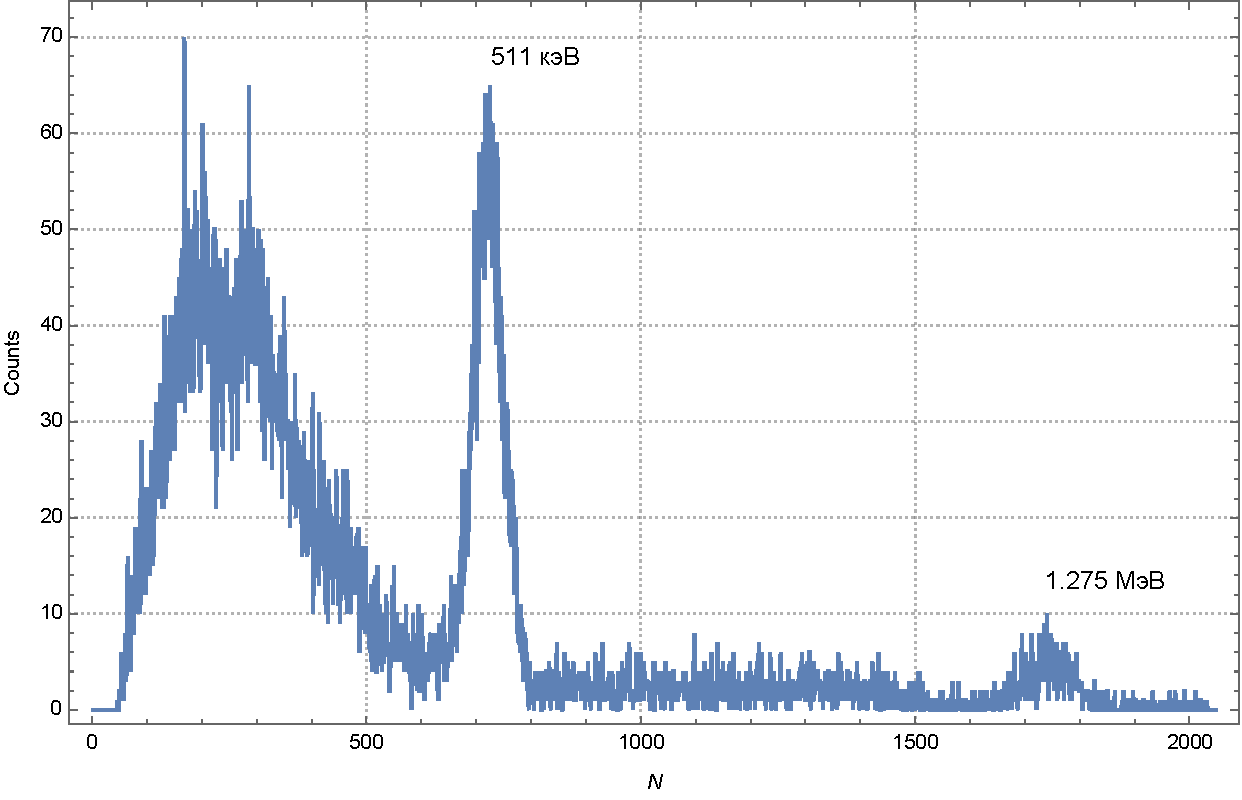
\includegraphics[scale=0.7]{calibration.pdf}
	 	\caption{Спектр $^{22}$Na}
	 \end{figure}
	 \par
	 Построим калибровочный график зависимости номера канала $N$ от энергии $\gamma$-кванта $E_i$. Предварительно аппроксимируем пики по функции Гаусса:
	 \begin{equation}
	 	y(x)=A\cdot e^{-\frac{(x-x_0)^2}{2*\sigma^2}}+B\cdot x+C
	 \end{equation}
	 Таким образом, спектр с аппроксимированными пиками имеет следующий вид:
	 \begin{figure}[!htb]
	 	\centering
	 	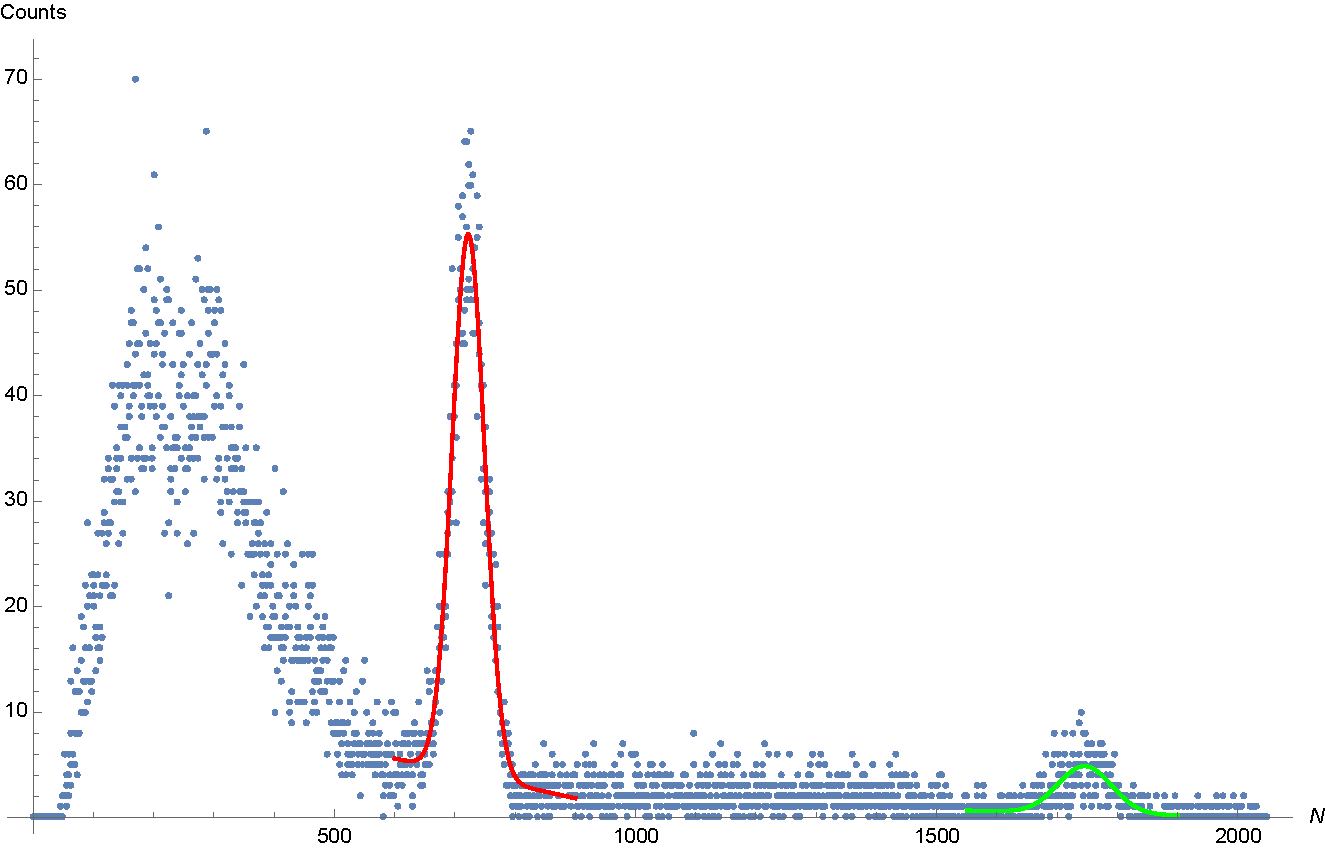
\includegraphics[scale=0.7]{calibration_approx.pdf}
	 	\caption{Спектр $^{22}$Na с аппроксимированными пиками}
	 \end{figure}
	 \par
	 Координаты пиков по горизонтальной оси соответсвтуют параметру $x_0$. Для данных пиков: $x_{01}=722.438$, $x_{02}=1746$. Тогда калибровочный график имеет вид:
	 \begin{figure}[!htb]
	 	\centering
	 	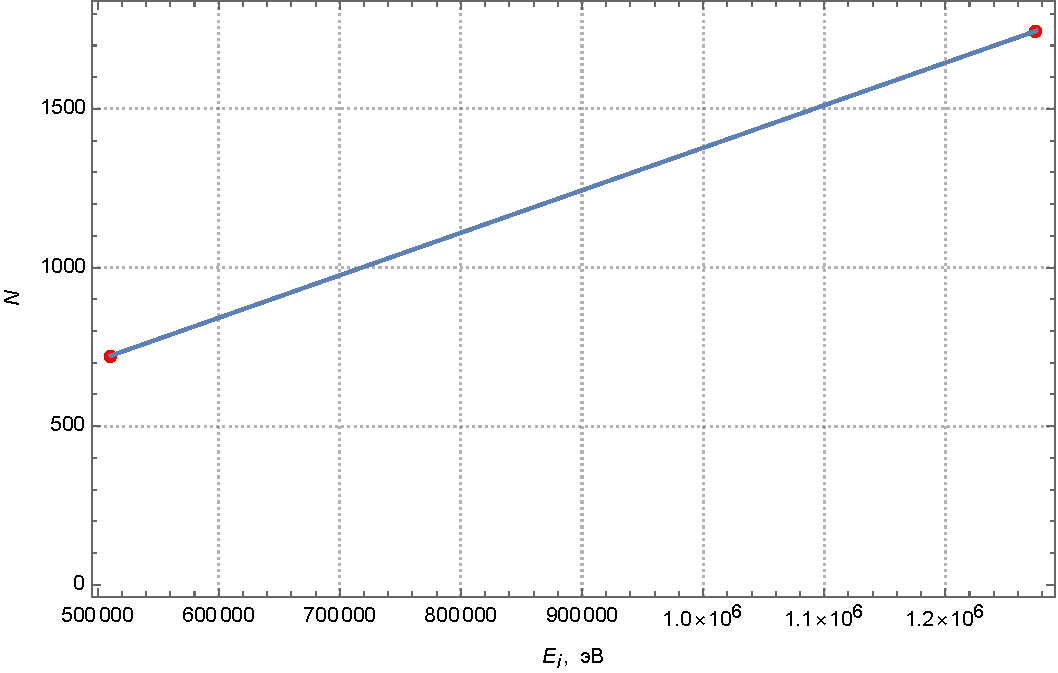
\includegraphics[scale=0.7]{calibrator.pdf}
	 	\caption{Калибровочный график}
	 \end{figure}
	 \par
	 Используя калибровочный график, определим для всех остальных источников значения энергии пиков полного поглощения $E_i$, их ширины на половине высоты $\Delta H_i$ и энергетическое разрешение $R_i$.
\end{document}